\section{Progress} \label{sec:progress}
Progress so far can be divided into two sections. Firstly, research has been made on the distinction between financial advice and guidance, the technologies to use for development, and the money management strategies. The second section is the development of a proof of concept web application, using the waterfall methodology, to demonstrate the feasibility of the project.

\subsection{Research}
\subsubsection{Financial Advice vs. Financial Guidance}
As outlined in the risks section of the project specification [\ref{appendix:project-specification}.6], a major factor to consider is distinguishing between financial advice and financial guidance; therefore this was heavily prioritised during the early stages of research.

As defined in the report from the Financial Conduct Authority (FCA) and HM Treasury \cite{FCAReport}, financial advice is defined as ``a service which recommends a specific course of action based on consumers' individual circumstances and goals''. This is in contrast to financial guidance, which is defined as ``provides information and/or options to narrow down consumers' choices, without making explicit recommendation''. These definitions are extremely reliable as the report is part of the Financial Advice Working Group's Review (FAWG), whose sole purpose is to demystify the differences and is what is considered in court.

It is important to consider this distinction when developing the application, as in the UK, it is illegal to provide financial advice on regulated investments without being vetted by the FCA's fact-find process \cite{FinancialAdviceLegalities}. In addition, the repercussions of providing financial advice include the potential that if a user were to lose money, they can sue the software for damages which is a major risk to consider \cite{SueBroker}. 

In particular, the application will be providing information specific to each user, as a result of using Plaid \cite{Plaid}, and so emphasis must be made that the strategies are not based on this, but rather are just general tools to help the user manage their money more effectively. An example an of implementation that follows is in the budgeting strategy. The user will be able to see their recent transactions, but they must opt in to begin budgeting and then set their strategy. The application will recommend the most effective strategy based on research later on in the project, but this will never be pushed onto the user.


\subsubsection{Technologies}
Also in accordance with the original timetable, research was conducted before development to help determine what technologies will be used. The main technologies that were considered were the web application framework, the database and the API for the bank connections.

Next.js was chosen as the frontend web application framework. It is a react-based framework that is extremely popular and has a large community. It is also very easy to use and has a lot of documentation. The project specification's non-function requirements were also considered when choosing the framework. For example, the requirement that the ``website must be fast to load and responsive to user input'' [\ref{appendix:project-specification}.3] is satisfied by Next.js as it has in-built functionality for server-side rendering and makes many optimisations by default \cite{NextjsPerformance}. Server-side rendering is when the more powerful server will render the page rather than the client; this means the pages feel faster and more responsive \cite{SSR}. Another requirement was that the application ``must be visually pleasing''. This will be accomplished by using TailwindCSS \cite{TailwindCSS}, a set of CSS classes that allows for complete customisation of the website's appearance without using a heavy component library.

To incorporate the users' bank data, Plaid was chosen as the API. It gives the most freedom to a user when specifying exactly what accounts are shared with the application; furthermore, they get peace of mind that their data is secure by Plaid using strict security measures such as end-to-end encryption and AES-256 with TLS \cite{Plaid}. The developer never sees or has to store the user's bank credentials as Plaid handles all of this, meaning the only data that is stored is the user's access token. This is stored in a secure database discussed in the next section. Moreover, Plaid has very detailed documentation and several tutorials on getting started \cite{PlaidGettingStarted}.

Originally, a full backend to perform the required server functionality was planned; however, after further research and understanding of the benefits of Next.js and Plaid, a conclusion of just using a simple database and performing all the querying using Next's API routes was made. Only the data for user authentication and a user's access token (or Plaid) needed to be stored, so a lightweight database was opted for. After comparing the various SQL and NoSQL alternatives, Pocketbase was the final decision thanks to its simplicity and ease of use \cite{NoBackendsPocketbase}. It is effectively a wrapper for SQLite, written in Go with a JavaScript SDK and REST API \cite{PocketbaseJavaScriptSDK}, so is the perfect choice for an application like this.

\subsubsection{Budgeting}
The budgeting strategy will be the first strategy to be developed as it is the most straightforward, and will be the easiest to demonstrate the feasibility of the project. This development is set to begin in a later phase of the project, but research has been conducted to help determine what the best budgeting approach is and how to implement it into the app already.

Budgeting is a concept that most would associate with money, but after reading some of the academic papers available such as \cite{hansen2003practice} and \cite{shim2011budgeting}, it is clear the budgeting can be applied to any type of resources such as time or energy. Furthermore, budgets can vary on a scale from personal to organisational; for example this book \cite{wildavsky1986budgeting} discusses how budgeting is carried out at a government level. This means that the best aspects of all types and scales can be applied to build the best strategy, and then implement it into the application.

So far some research has gone into finding which budgeting approach and the current conclusion is to do the 50/30/20 strategy. This is where an individual separates their monthly income into 50\% for needs, 30\% for wants and 20\% for savings or repaying debt \cite{503020Strategy}. It originates from the book ``All Your Worth: The Ultimate Lifetime Money Plan'' \cite{warren2005all} which itself references over 20 years of research. It is considered the best approach for the web application as it is simple to understand, yet effective according to many studies \cite{503020Examples}; on top of that, it is also considered very appropriate for the current cost of living crisis over other methods like the digital envelope approach \cite{503020InCostLivingCrisis}.

The implementation of this 50/30/20 strategy is also somewhat simple, as users will be able to opt in to let the software calculate how much money is assigned to each section. Furthermore, it would be possible to let users categorise their previous transactions into these and determine how they would need to change their previous spending habits to match. Also, they could have the 20\%, that is used to repay debt and save, automatically accounted for in a separate loans section of the application.

The research at this stage is not final and other options are still being considered, however, the 50/30/20 strategy is the current favourite. As a result of performing the second phase of development in sprints, it will be possible to test the effectiveness of the strategy and make changes if necessary without majorly affecting the project timeline.

\subsection{Development}
The development of the proof of concept web application is using the waterfall methodology - a sequential approach to software development. This is enabled as the requirements are well defined and there is a clear end goal. So far, two separate concepts have been developed. The first is the basic authentication system using Next.js, TailwindCSS and Pocketbase. It is currently working and passing all the unit tests that have been written. The second is the Plaid integration, where the quickstart project has been set up and is currently working with some slight adjustments. The next step is to combine the two concepts and then move on to repeated strategy implementation.

The below figures are screenshots of the Plaid proof of concept. They simulate the users actions after landing on the first page. Firstly they open the link pop-up; then, they choose which bank to connect to; after that, they log into their institution securely; then, they select which accounts to sync; and finally, they can view centralised information about them all, including recent transactions.

\begin{figure}[H]
    \centering
    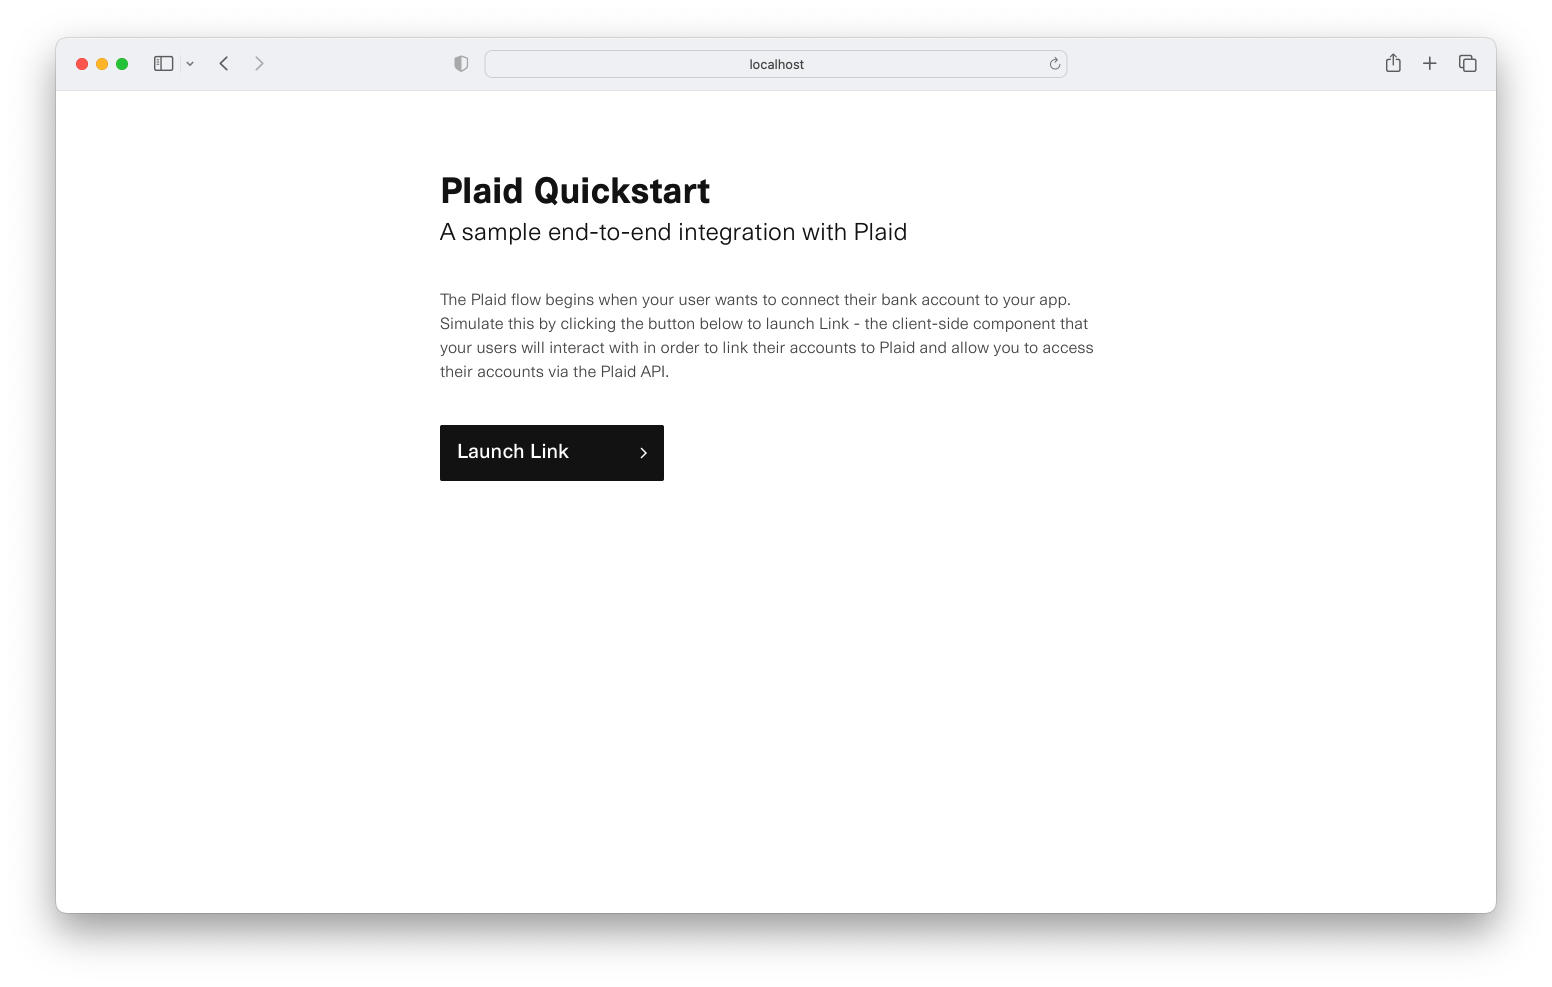
\includegraphics[scale=0.53]{landing_page.png}
	\vspace{-0.8cm}
    \caption{The landing page of the Plaid PoC}
	\label{fig:landing_page}
\end{figure}
    
\begin{figure}[H]
	\centering
    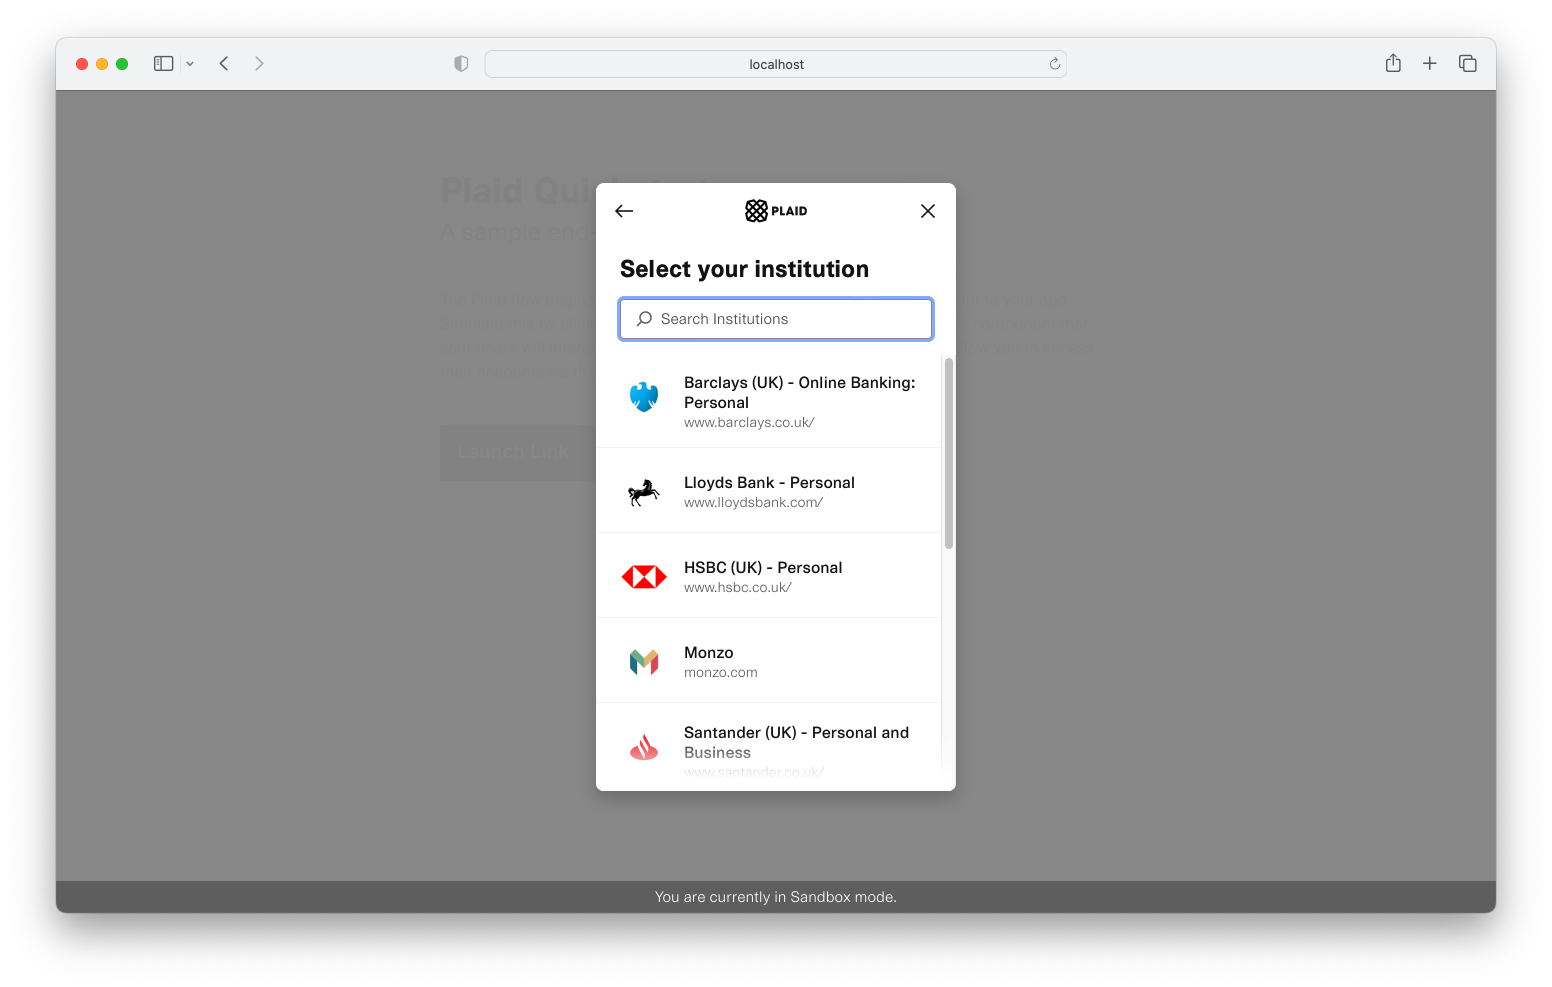
\includegraphics[scale=0.53]{bank_search.png}
	\vspace{-0.8cm}
    \caption{Simulating a user choosing which bank to connect to}
    \label{fig:bank_search}
\end{figure}

\begin{figure}[H]
	\centering
    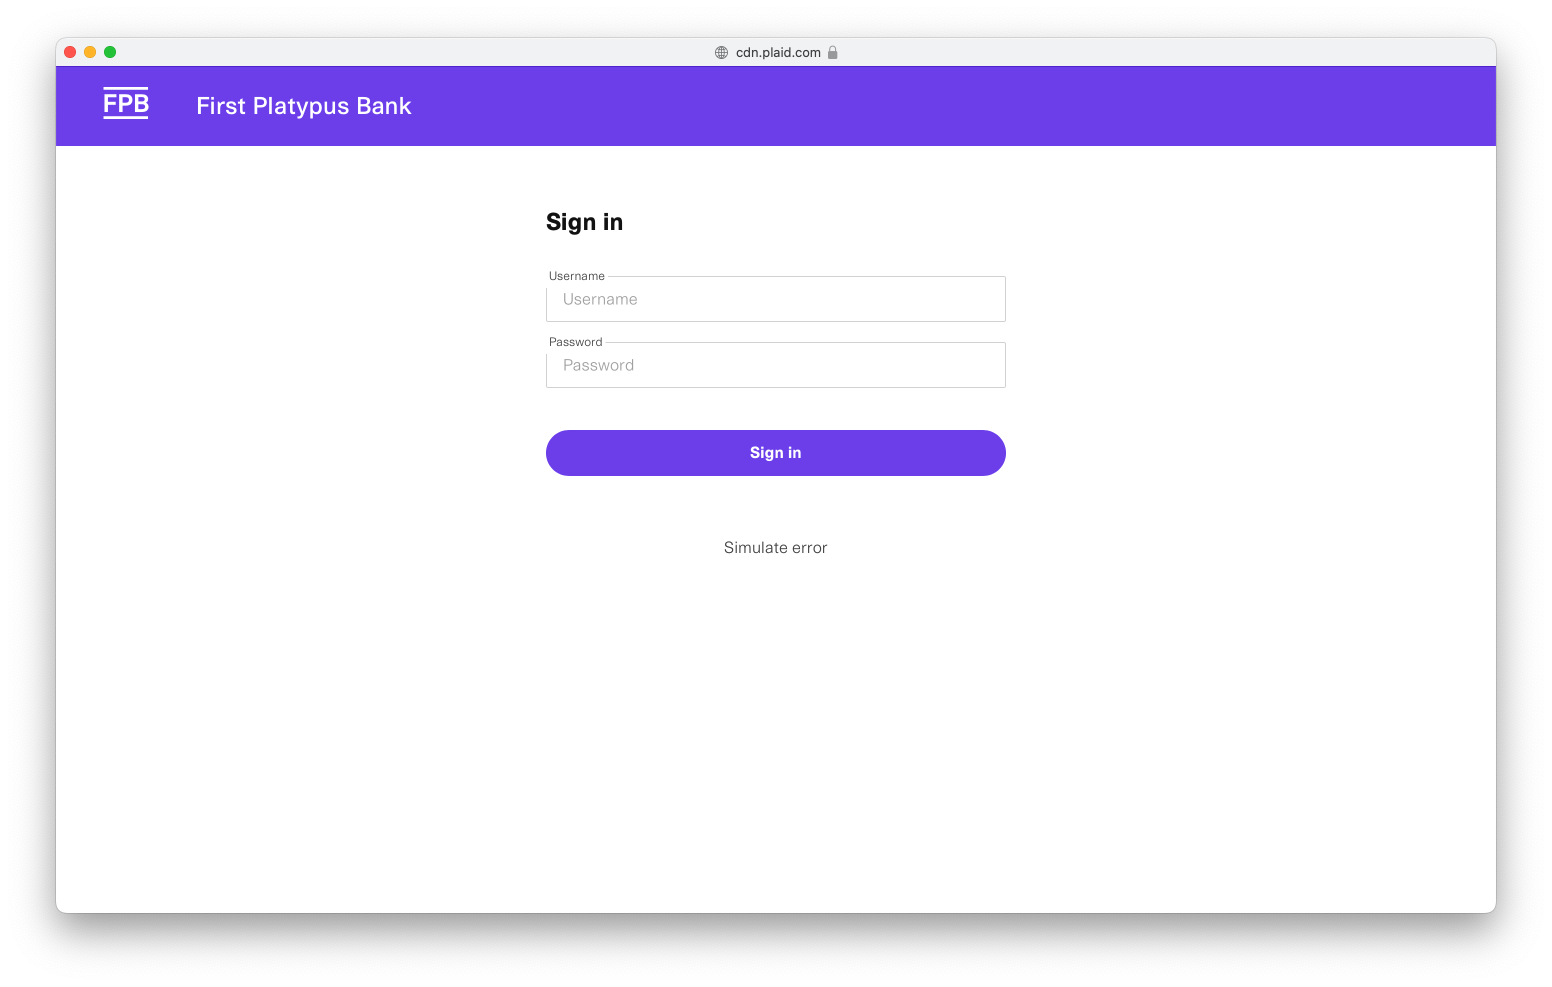
\includegraphics[scale=0.53]{bank_login.png}
	\vspace{-0.8cm}
    \caption{Simulating a user choosing logging into their bank}
    \label{fig:bank_login}
\end{figure}

\begin{figure}[H]
	\centering
    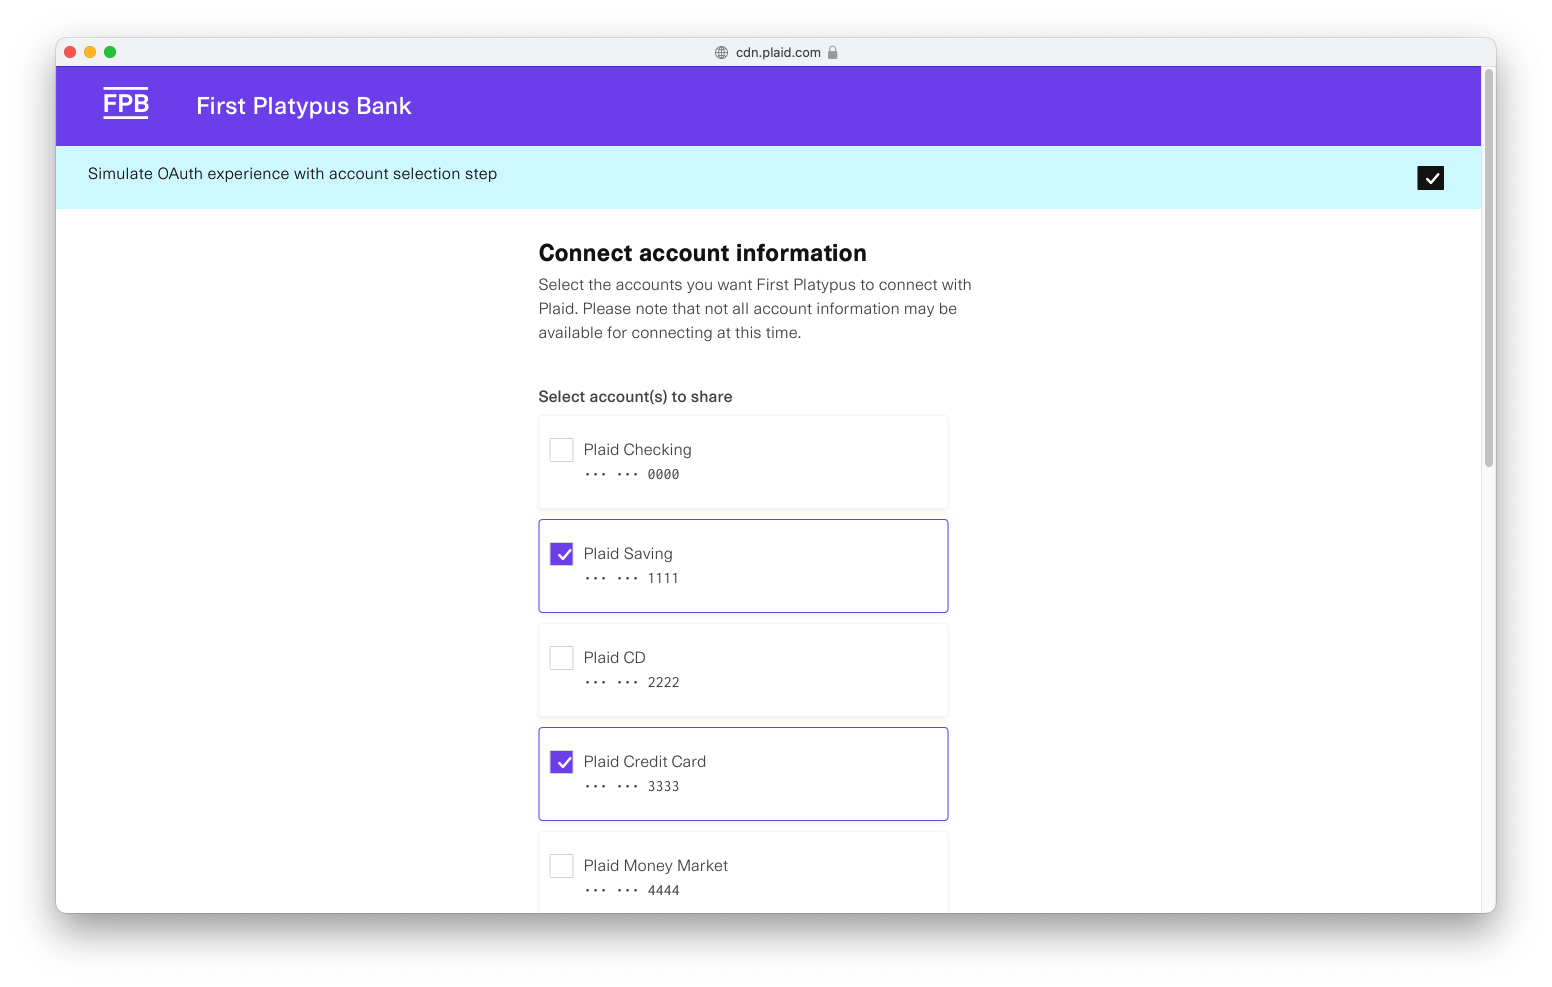
\includegraphics[scale=0.53]{account_choice.png}
	\vspace{-0.8cm}
    \caption{Simulating an authenticated user choosing which accounts to link}
    \label{fig:account_choice}
\end{figure}

\begin{figure}[H]
	\centering
    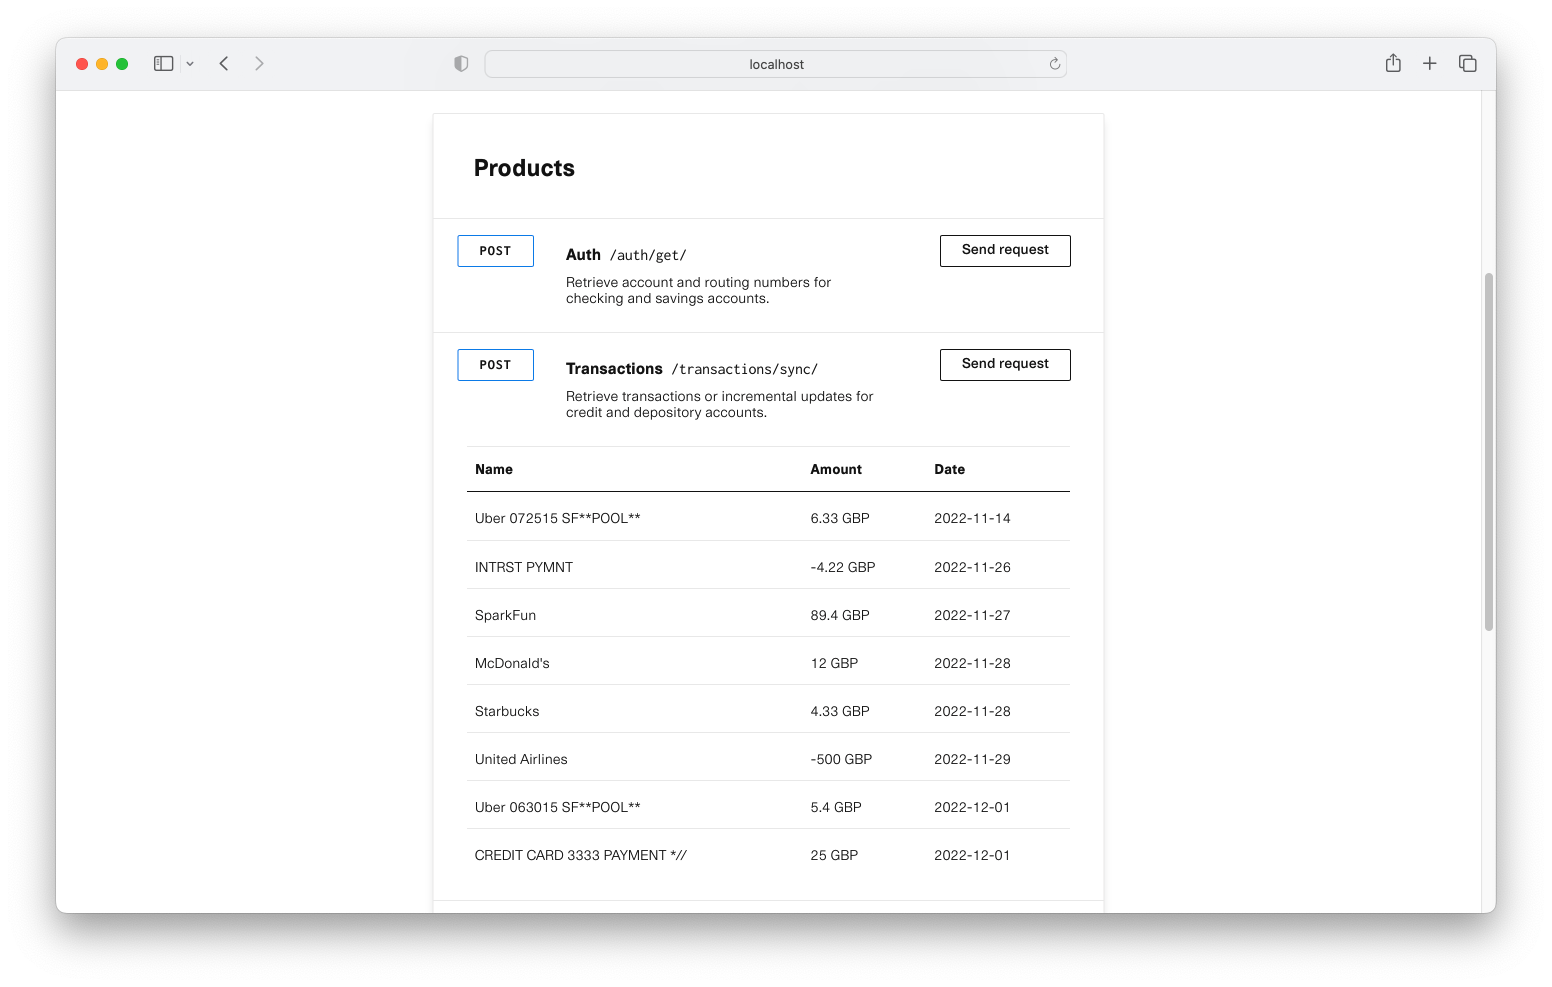
\includegraphics[scale=0.53]{transactions.png}
	\vspace{-0.8cm}
    \caption{Simulating an authenticated user viewing their transactions}
    \label{fig:transactions}
\end{figure}

